\documentclass[3p,twocolumn,authoryear]{elsarticle}

\usepackage{natbib}
\usepackage{algorithm}
\usepackage{algpseudocode}
\usepackage{booktabs}
\usepackage{graphicx}
\usepackage{amsmath}
\usepackage{lineno}
% \modulolinenumbers[5]   % uncomment for line numbers during review

\journal{Artificial Intelligence in Agriculture}

%% ─── Bibliography style: author-year ────────────────────────────────────────
\bibliographystyle{elsarticle-harv}

\begin{document}

\begin{frontmatter}

\title{An Explainable AI-based Decision Support System for Precision
       Allocation of Agricultural Skill Development Programs}

%% TODO: Replace with actual author names and affiliations
\author[inst1]{[First Author Name]\corref{cor1}}
\ead{[email@university.ac.th]}

\author[inst1]{[Co-author Name]}

\cortext[cor1]{Corresponding author}
\affiliation[inst1]{organization={[Department, University Name]},
             addressline={[Address]},
             city={[City]},
             country={Thailand}}

%%─── Abstract ────────────────────────────────────────────────────────────────
\begin{abstract}
Precision allocation of agricultural skill development programs
remains a challenge due to the systematic heterogeneity of farmer
populations and the limitations of one-size-fits-all training designs.
This study proposes an explainable AI-based decision support system
(DSS) for targeting training interventions across diverse farmer
segments.
The framework integrates K-Means clustering for farmer segmentation,
Random Forest regression for skill outcome modeling, and
SHapley Additive exPlanations (SHAP) for interpretable feature
attribution, organized within a unified
Segment--Attribute--Recommend (SAR) pipeline.
Applied to panel survey data from $n = 833$ participants in
Thailand's Smart Farmer program, the framework identifies three
structurally meaningful farmer segments---Low-skill, Moderate-skill,
and High-skill---and reveals that overall skill level, production
management competency, and educational attainment are the primary
determinants of training effectiveness.
Cluster-level SHAP analysis further demonstrates that the relative
importance of these predictors varies systematically across segments,
confirming that global feature importance is insufficient for
precision training design.
A surrogate decision tree (accuracy = 93.3\%) translates
SHAP-derived attributions into transparent IF--THEN rules,
enabling agricultural extension practitioners to implement
data-driven training recommendations without requiring direct
interaction with the underlying machine learning system.
The proposed SAR architecture provides a deployable and
generalizable framework for AI-driven human capital development
in agricultural extension systems.
\end{abstract}

\begin{keyword}
Explainable AI \sep SHAP \sep Decision Support System \sep
Farmer Segmentation \sep Agricultural Extension \sep Machine Learning
\end{keyword}

\end{frontmatter}

% \linenumbers   % uncomment for line numbers during review

%%─────────────────────────────────────────────────────────────────────────────
\section{Introduction}
%%─────────────────────────────────────────────────────────────────────────────

The rapid advancement of artificial intelligence (AI) has transformed
agricultural systems from input-driven production models into
data-driven decision ecosystems.
While smart agriculture technologies have primarily focused on
optimising physical processes such as crop monitoring, irrigation,
and yield prediction, comparatively less attention has been devoted
to AI-driven systems that support human capital
formation---a critical determinant of long-term agricultural
productivity and resilience.

Agricultural skill development programs represent one of the most
widely implemented instruments for improving farmer performance.
However, their effectiveness remains constrained by the uniform
allocation of training interventions across heterogeneous farmer
populations.
Farmers differ systematically in baseline competencies, risk
perception, resource access, and learning readiness, yet
standardised curricula are commonly applied across all participants.
This mismatch results in inefficient resource allocation and
suboptimal learning outcomes \citep{anderson2004,feder1985}.
Critically, training effectiveness is a direct precursor to
technology adoption: farmers who acquire targeted skills are more
likely to adopt precision irrigation, integrated pest management,
and market-oriented practices \citep{davis2012}---all of which
underpin the productivity gains that smart agriculture promises.

Recent advances in machine learning (ML) \citep{kamilaris2018,
liakos2018,yang2025} enable modelling of complex and non-linear
relationships within agricultural datasets, offering new
opportunities to predict heterogeneous outcomes across individuals.
However, predictive capability alone is insufficient for real-world
deployment.
Decision-making in agricultural extension requires transparency,
interpretability, and actionable logic that practitioners can
operationalise.
This has led to increasing interest in explainable artificial
intelligence (XAI) \citep{arrieta2020,ryo2022}, particularly
SHapley Additive exPlanations (SHAP), which provides
theoretically grounded feature attribution for tree-based models
\citep{lundberg2017}.
Despite these advances, a critical gap remains: the absence of
integrated AI frameworks that translate predictive and explainable
insights into structured, deployable decision support systems for
agricultural training design.

This study addresses this gap by proposing an explainable
AI-based Decision Support System (DSS) for precision allocation of
agricultural skill development programs.
The framework integrates K-Means clustering, Random Forest
regression, and SHAP analysis within a unified
Segment--Attribute--Recommend (SAR) pipeline.
Unlike prior studies that treat explainability as a post-hoc
interpretive tool, this study operationalises SHAP outputs as the
foundation for generating explicit decision rules via a surrogate
decision tree, enabling the transition from predictive analytics
to actionable decision intelligence.

The study is guided by three research questions:
(1) Can unsupervised learning methods identify structurally
meaningful farmer segments for training design?
(2) Can machine learning models provide sufficient predictive
structure to support SHAP-based interpretation in skill development
contexts?
(3) How can SHAP-based explanations be transformed into
interpretable and implementable decision rules for agricultural
extension systems?

This study makes three primary contributions.
First, it extends AI beyond predictive analytics toward actionable
decision-making via an integrated DSS for human capital development.
Second, it advances XAI by introducing a cluster-level SHAP approach
that links model interpretability to structured decision logic.
Third, it proposes a deployable SAR architecture that transforms
model outputs into transparent, auditable decision rules via a
surrogate decision tree, enabling practical implementation by
domain practitioners.

All findings are interpreted as associative; the observational
dataset does not support causal inference.

%%─────────────────────────────────────────────────────────────────────────────
\section{Literature Review}
%%─────────────────────────────────────────────────────────────────────────────

\subsection{Farmer Heterogeneity and Training Effectiveness}

A long-standing insight in agricultural economics is that farmers
are far from homogeneous.
Variations in human capital, resource endowments, and access to
information shape both productivity and technology adoption, causing
standardised training programs to deliver uneven outcomes
\citep{feder1985}.

Empirical studies consistently show that farmers with stronger
baseline skills tend to gain more from advanced training, while
those starting with lower capabilities find complex content
difficult to absorb \citep{davis2012}.
Training effectiveness is therefore closely tied to individual
characteristics, underscoring the importance of tailoring
interventions rather than relying on uniform approaches.
Despite this evidence, many extension systems continue to implement
one-size-fits-all programs due to operational constraints and the
absence of systematic targeting tools \citep{anderson2004}.

\subsection{Machine Learning in Agriculture}

Machine learning has gained substantial traction in the agricultural
domain \citep{kamilaris2018,liakos2018}, with applications spanning
crop yield prediction, disease detection, and resource optimisation.
Ensemble models such as Random Forest and gradient boosting are
particularly prominent owing to their strong performance on
structured agricultural datasets.

AI-driven systems have also demonstrated potential for automating
operational tasks: quality inspection and classification systems
have been found to improve accuracy and consistency relative to
manual processes \citep{wonggasem2024}.
Nevertheless, most existing studies remain focused on production and
environmental outcomes, with limited attention to human capital
development and training systems.
Moreover, many machine learning applications emphasise prediction
without addressing how model outputs can be translated into
actionable decisions, limiting their practical usefulness
\citep{ryo2022}.

\subsection{Explainable AI and Decision Support Systems}

As machine learning models become more complex, interest in
explainable artificial intelligence (XAI) has grown accordingly
\citep{arrieta2020,lipton2018}.
SHAP has emerged as a widely used approach for interpreting
tree-based models due to its theoretical grounding and its ability
to provide both global and local explanations \citep{lundberg2017}.
SHAP decomposes model predictions into feature-level contributions,
enabling users to understand not only which variables matter but
also how they influence outcomes.

Despite these advances, integrating XAI into operational
decision-making remains limited.
Most studies focus on interpretation alone, without a clear pathway
for converting model explanations into structured decision rules.
This study addresses that gap by linking SHAP analysis with
segmentation and surrogate rule extraction to produce a decision
support system that is both practical and deployable
\citep{yang2025,zhang2026}.

%%─────────────────────────────────────────────────────────────────────────────
\section{Methodology}
%%─────────────────────────────────────────────────────────────────────────────

\subsection{Data and Study Context}

The dataset consists of panel survey data from $n = 833$ farmers
participating in the Smart Farmer program in Thailand.
Observations capture pre- and post-training measurements including
demographic characteristics, resource access, risk perception, and
multiple dimensions of agricultural skills.
The primary outcome variable is the change in overall skill score,
$Ch\_Skill$, defined as the difference between post-training and
pre-training composite scores.

Missing values were addressed using simple imputation: binary and
asset-related variables were imputed with zero; continuous variables
were imputed with column means.
All numeric predictors were standardised to zero mean and unit
variance prior to modelling.

\subsection{Farmer Segmentation}

Farmer heterogeneity was addressed using K-Means clustering
applied to 15 baseline features spanning skill levels,
demographics, and risk indicators.
The optimal number of clusters was determined using the combined
evidence of the Elbow method and Silhouette analysis
\citep{rouseeuw1987}.
As shown in Fig.~\ref{fig:elbow}, the Elbow curve exhibits a
pronounced inflection at $k = 3$, indicating a meaningful
gain in within-cluster homogeneity relative to complexity.
The Silhouette score at $k = 3$ is 0.185, which, while modest,
is consistent with the overlapping nature of social survey data
that rarely exhibits the compact, spherical cluster structure
assumed by metrics such as Silhouette or Davies-Bouldin.
Notably, Silhouette scores are consistently low across all values
of $k$ (range: 0.14--0.20), indicating that weak separation is
a property of the data rather than a specific choice of $k$.
The selection of $k = 3$ is further supported by domain knowledge:
Thailand's Smart Farmer program operates with three formal
proficiency tiers (Smart Farmer, Smart Farmer in Progress,
and Knowledge Farmer), making a three-segment structure directly
actionable in the extension context.

\subsection{Predictive Modelling}

A Random Forest regression model \citep{breiman2001} was employed
to predict $Ch\_Skill$, using 18 features spanning demographic
characteristics, baseline skills, risk perception, and program
participation.
All models were estimated via 5-fold cross-validation.
XGBoost \citep{chen2016} was included as a robustness check.

\subsection{Baseline Models and Performance Evaluation}

Two baseline models---ordinary least squares (OLS) linear
regression and ridge regression---were estimated using the same
feature set to provide a transparent benchmark.
Performance was evaluated using $R^{2}$, root mean squared error
(RMSE), and mean absolute error (MAE) under 5-fold cross-validation.
Table~\ref{tab:baseline_performance} reports the results.

The Random Forest (optimised via grid search:
\texttt{n\_estimators}=500, \texttt{min\_samples\_leaf}=10,
\texttt{max\_features}=\texttt{sqrt}) achieves $R^{2} = 0.213$,
outperforming the linear and ridge baselines ($R^{2} = 0.185$
and $0.186$, respectively).
The modest absolute $R^{2}$ values across all models reflect the
inherent stochasticity of human learning outcomes and the
influence of unobserved motivational factors common in
observational survey data.
Importantly, the value of the Random Forest in this study lies
in its structural capacity to model non-linear threshold effects
and feature interactions---the prerequisite for meaningful
SHAP analysis and surrogate rule extraction developed in
subsequent sections.

\begin{table}[htbp]
\centering
\caption{5-fold cross-validated model performance for predicting
         skill improvement (\textit{Ch\_Skill}), $n = 833$.}
\label{tab:baseline_performance}
\begin{tabular}{@{}lccc@{}}
\toprule
\textbf{Model} & \textbf{$R^{2}$} & \textbf{RMSE} & \textbf{MAE} \\
\midrule
Linear Regression  & 0.185 & 0.615 & 0.492 \\
Ridge Regression   & 0.186 & 0.614 & 0.492 \\
\textbf{Random Forest (ours)} & \textbf{0.213} & \textbf{0.607} & \textbf{0.476} \\
\bottomrule
\end{tabular}
\end{table}

\subsection{Explainable AI Analysis}

SHAP values were computed for all observations using
\texttt{shap.TreeExplainer} \citep{lundberg2017} to quantify
the marginal contribution of each feature to the Random Forest
predictions.
Global feature importance was derived as mean absolute SHAP values
across all observations.
SHAP analysis was subsequently conducted at the cluster level to
identify segment-specific drivers of skill improvement,
constituting the Attribute stage of the SAR pipeline.

\subsection{Decision Support Framework}

The proposed DSS follows a three-stage SAR architecture
(Fig.~\ref{fig:framework}).
In the \textit{Segment} stage, farmers are assigned to one of
three groups via K-Means clustering.
In the \textit{Attribute} stage, cluster-level SHAP values
identify the most influential predictors within each segment.
In the \textit{Recommend} stage, a surrogate decision tree
encodes these attributions into interpretable IF--THEN rules
for training allocation.

\subsection{Rule Extraction Method}

Decision rules are extracted in two steps.
In Step~1 (feature selection), mean absolute SHAP values within
each cluster identify \textit{which} features to include as
rule conditions.
In Step~2 (threshold calibration), a surrogate decision tree
(depth = 3) is fitted on the SHAP-selected features to derive
data-driven classification thresholds.
This two-step process ensures that rules are simultaneously
grounded in SHAP attribution theory and empirically
calibrated to the data distribution.

The procedure is summarised in Algorithm~\ref{alg:rules}.

\begin{algorithm}
\caption{SHAP-guided Surrogate Rule Extraction}
\label{alg:rules}
\begin{algorithmic}[1]
\Require Cluster assignments $C$, SHAP matrix $S$,
         feature matrix $X$, tree depth $d$
\Ensure Set of IF--THEN rules $\mathcal{R}$
\State $\mathcal{R} \gets \emptyset$
\For{each cluster $c$ in $C$}
    \State $\phi_j \gets \text{mean}(|S_{c,j}|)$
           \Comment{Mean abs.\ SHAP per feature}
    \State $\mathcal{F}_c \gets \text{Top-}K(\phi)$
    \State Fit surrogate tree $T_c$ on $X[\mathcal{F}_c]$
           with depth $d$
    \State Extract rules $\mathcal{R}_c$ from $T_c$ leaf paths
    \State $\mathcal{R} \gets \mathcal{R} \cup \mathcal{R}_c$
\EndFor
\State \Return $\mathcal{R}$
\end{algorithmic}
\end{algorithm}

\subsection{Clustering Robustness}

Alternative cluster counts ($k = 2$--$8$) were explored.
The dominant features defining each segment and the qualitative
distinctions among the Low-skill, Moderate-skill, and High-skill
groups remained stable across all tested values of $k$,
supporting the reliability of the segmentation within the
SAR pipeline.

%%─────────────────────────────────────────────────────────────────────────────
\section{Results}
%%─────────────────────────────────────────────────────────────────────────────

\subsection{Farmer Segmentation}

The K-Means algorithm ($k = 3$) identifies three distinct
farmer segments, visualised via PCA in
Fig.~\ref{fig:clusters}.
Table~\ref{tab:cluster_profile} reports the mean profile
of each segment.

The \textbf{Low-skill} cluster ($n = 271$) comprises older
farmers (mean age 54.9 years) with the lowest educational
attainment (mean edu = 2.9) and the weakest baseline skills
across all dimensions.
Notably, this segment shows a negative mean skill change
($Ch\_Skill = -0.233$), which is consistent with a
regression-to-the-mean effect: farmers with the lowest
baseline scores are most susceptible to measurement
instability and ceiling-floor artefacts in repeated
assessments \citep{davis2012}.
This finding reinforces the need for foundational, scaffolded
training designs for this segment rather than assuming uniform
improvement.

The \textbf{Moderate-skill} cluster ($n = 228$) shows
intermediate baseline capabilities and the highest market
risk perception (mean = 3.23), reflecting exposure to
market-facing agricultural activities.
The near-zero skill change ($Ch\_Skill = -0.105$) suggests
that standard training content is insufficient to produce
measurable gains in this group, indicating a need for
differentiated, context-sensitive program design.

The \textbf{High-skill} cluster ($n = 334$) exhibits
the strongest baseline competencies, the highest Smart
Farmer participation rate (69.8\%), and the only positive
mean skill change ($Ch\_Skill = +0.259$).
This pattern suggests a reinforcing dynamic: farmers with
strong pre-training capabilities are better positioned to
absorb and apply training content.

\begin{table*}[htbp]
\centering
\caption{Cluster profile: mean variable values by farmer segment
         ($n = 833$). Skill scales: 1--5 Likert.}
\label{tab:cluster_profile}
\begin{tabular}{@{}lcccccccc@{}}
\toprule
\textbf{Segment} & \textbf{n} & \textbf{All\_Skill}
  & \textbf{Ch\_Skill} & \textbf{Age}
  & \textbf{Education} & \textbf{ProdManage}
  & \textbf{Tech} & \textbf{SF Rate} \\
\midrule
Low-skill      & 271 & 3.06 & $-$0.233 & 54.9 & 2.9 & 3.58 & 3.05 & 28.8\% \\
Moderate-skill & 228 & 3.26 & $-$0.105 & 50.6 & 3.8 & 3.42 & 3.22 & 51.3\% \\
High-skill     & 334 & 4.27 & $+$0.259 & 52.6 & 3.7 & 4.46 & 4.40 & 69.8\% \\
\bottomrule
\end{tabular}
\end{table*}

\subsection{Predictive Performance}

The optimised Random Forest achieves $R^{2} = 0.213$
(Table~\ref{tab:baseline_performance}), outperforming both
linear and ridge regression baselines.
Modest $R^{2}$ values across all models are expected in
observational studies of human learning: skill change is
influenced by unobserved motivational, contextual, and
interpersonal factors that cannot be captured in a
cross-sectional feature set.
The XGBoost model yields comparable performance
($R^{2} \approx 0.21$), supporting the robustness of the
predictive component.

\subsection{SHAP-Based Global Feature Importance}

Fig.~\ref{fig:importance} presents global SHAP-based feature
importance across all $n = 833$ observations.
Overall skill level (\texttt{All\_Skill}) emerges as the
dominant predictor by a substantial margin, followed by
production management skills (\texttt{Avg\_ProdManage}),
education (\texttt{edu}), marketing skills
(\texttt{Avg\_Mkting}), and irrigation access
(\texttt{irriga}).

The dominance of \texttt{All\_Skill} is consistent with
human capital theory: farmers with stronger pre-training
competencies are better positioned to absorb new knowledge
\citep{feder1985}.
The secondary contributions of production management and
education suggest that technical capability and formal
educational background moderate training uptake.
Notably, training-type variables contribute minimally to
model predictions, indicating that what farmers bring to
training---their existing capabilities and contextual
resources---is a stronger determinant of outcomes than the
specific training modality received.

\subsection{SHAP Beeswarm Analysis}

The SHAP beeswarm plot (Fig.~\ref{fig:shap}) reveals the
distributional patterns of feature contributions across
individual observations.
For \texttt{All\_Skill}, high feature values (red) are
associated with strongly positive SHAP contributions,
while low values (blue) produce strongly negative
contributions, indicating a near-monotonic positive
relationship with a range of approximately $-1.25$ to
$+1.25$.
For \texttt{irriga}, the predominantly negative
contributions suggest that farmers with irrigation
access may already hold higher pre-training baselines,
yielding smaller measured improvement.
These non-linear, heterogeneous patterns confirm that
the model captures structural relationships that linear
regression coefficients cannot represent.

\subsection{Cluster-Level SHAP Analysis}

Fig.~\ref{fig:clusterShap} presents cluster-stratified
SHAP beeswarm plots for the three farmer segments.
While \texttt{All\_Skill} remains the dominant feature
across all clusters, the relative importance of secondary
features varies systematically.

In the \textbf{Low-skill} cluster, \texttt{Avg\_ProdManage}
and \texttt{edu} show pronounced negative contributions
for low-value observations, indicating that deficits
in production management and educational attainment are
particularly constraining for skill improvement in this
segment.
In the \textbf{Moderate-skill} cluster, contribution
patterns are more symmetric, reflecting joint influences
from multiple factors.
In the \textbf{High-skill} cluster, \texttt{Avg\_Mkting}
rises in relative importance, suggesting that
market-oriented competencies become a binding constraint
on further advancement among already high-performing farmers.

These segment-specific patterns support differentiated
training intervention design and confirm that global
feature importance is insufficient for precision training
allocation.

\subsection{Decision Rule Extraction}

A surrogate decision tree (depth = 3) fitted on
SHAP-selected features achieves a classification accuracy
of 93.3\% on the full dataset ($n = 833$, Fig.~\ref{fig:rules}).

The root split at \texttt{All\_Skill} $\leq 3.005$
partitions farmers into a lower-potential group
(223 farmers, 26.8\%) and a higher-potential group
(610 farmers, 73.2\%).
Within the lower-potential branch, a secondary split on
\texttt{Avg\_Mkting} $\leq 3.5$ further separates farmers
by marketing skill level.
Within the higher-potential branch, a split at
\texttt{All\_Skill} $\leq 4.255$ distinguishes
moderate-high from high-performing farmers,
directing the latter toward advanced and
market-oriented interventions.

These data-calibrated thresholds translate SHAP-derived
feature importance into transparent, auditable IF--THEN
rules that extension practitioners can apply without
direct interaction with the machine learning system.

\begin{figure}[htbp]
\centering

\includegraphics[width=\columnwidth]{figures/fig1_framework.png}
\caption{The proposed Segment--Attribute--Recommend (SAR)
         decision support framework integrating K-Means
         segmentation, Random Forest modelling, and
         SHAP-based explanation into a unified pipeline for
         agricultural skill development.}
\label{fig:framework}
\end{figure}

\begin{figure}[htbp]
\centering
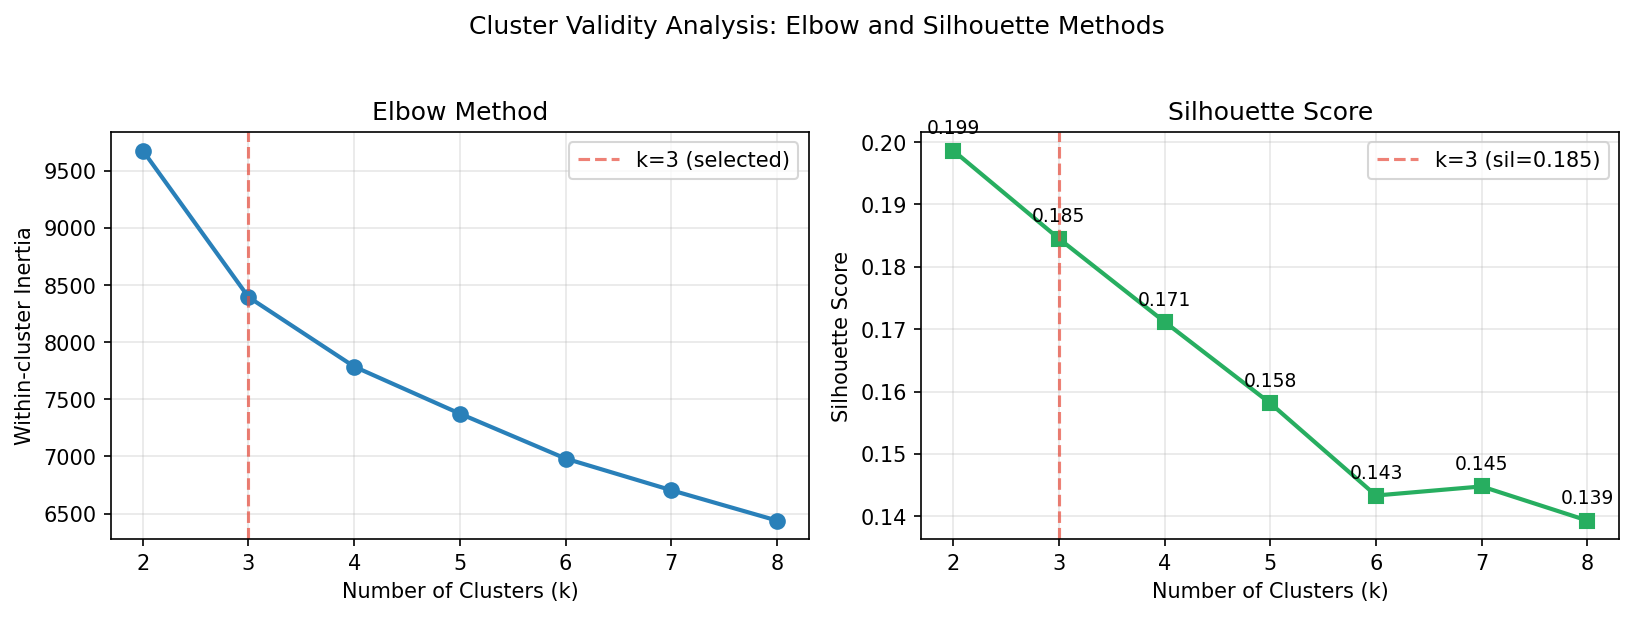
\includegraphics[width=\columnwidth]{figures/fig_elbow_silhouette.png}
\caption{Cluster validity analysis: Elbow method (left) and
         Silhouette score (right) for $k = 2$--$8$.
         The Elbow curve exhibits a pronounced inflection at
         $k = 3$; Silhouette scores are uniformly low across
         all $k$ values, reflecting the overlapping structure
         characteristic of social survey data.
         Domain alignment with Thailand's three-tier Smart
         Farmer proficiency system provides additional
         justification for $k = 3$.}
\label{fig:elbow}
\end{figure}

\begin{figure}[htbp]
\centering
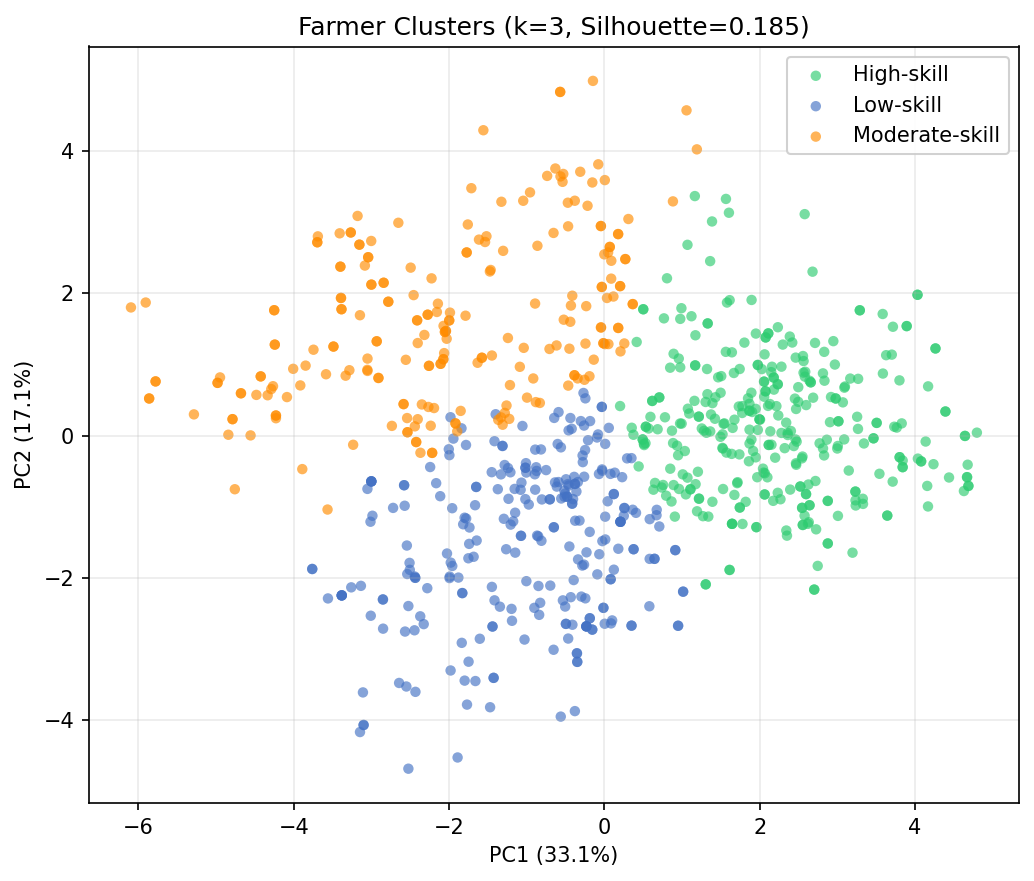
\includegraphics[width=\columnwidth]{figures/fig2_clusters_new.png}
\caption{Farmer segmentation via K-Means ($k = 3$, Silhouette
         = 0.185), visualised in PCA space.
         Three segments---Low-skill (blue), Moderate-skill
         (orange), and High-skill (green)---reflect systematic
         differences in baseline competencies, educational
         attainment, and resource access (see
         Table~\ref{tab:cluster_profile}).}
\label{fig:clusters}
\end{figure}

\begin{figure}[htbp]
\centering
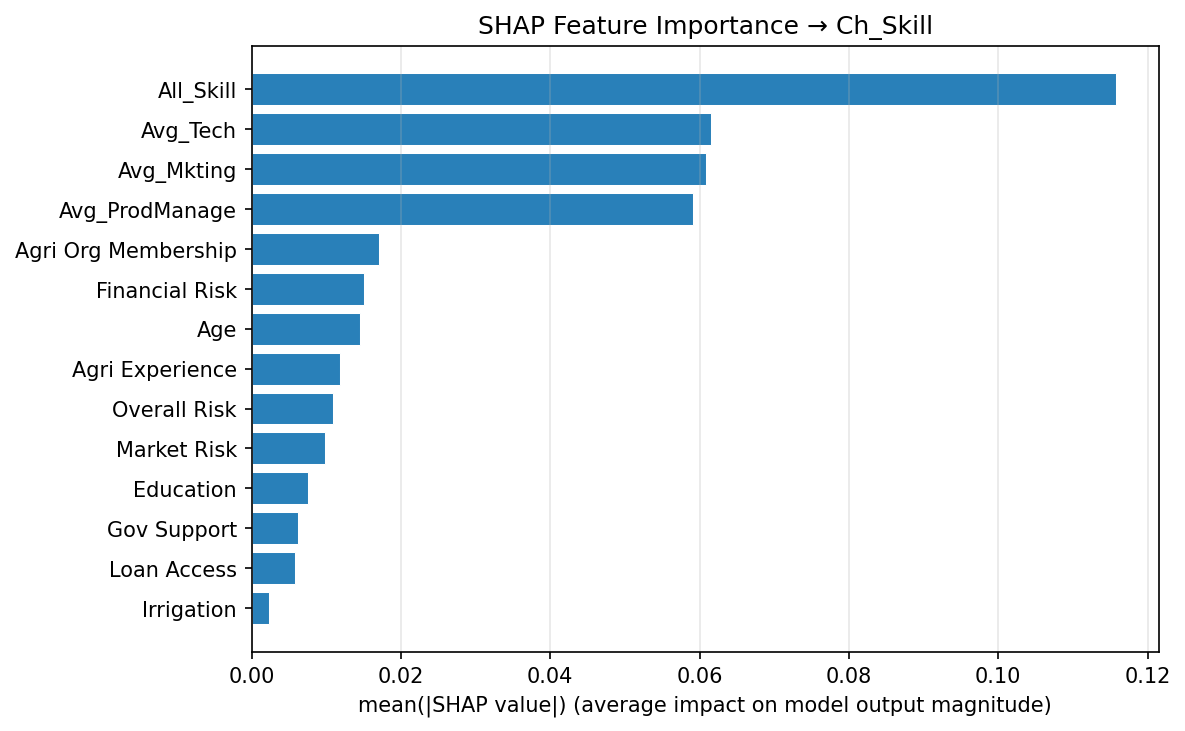
\includegraphics[width=\columnwidth]{figures/fig3_importance_new.png}
\caption{Global SHAP-based feature importance (mean
         $|\text{SHAP value}|$) across all observations
         ($n = 833$).
         Overall skill level (\texttt{All\_Skill}) is the
         dominant predictor, followed by production
         management, education, marketing skills, and
         irrigation access.}
\label{fig:importance}
\end{figure}

\begin{figure}[htbp]
\centering
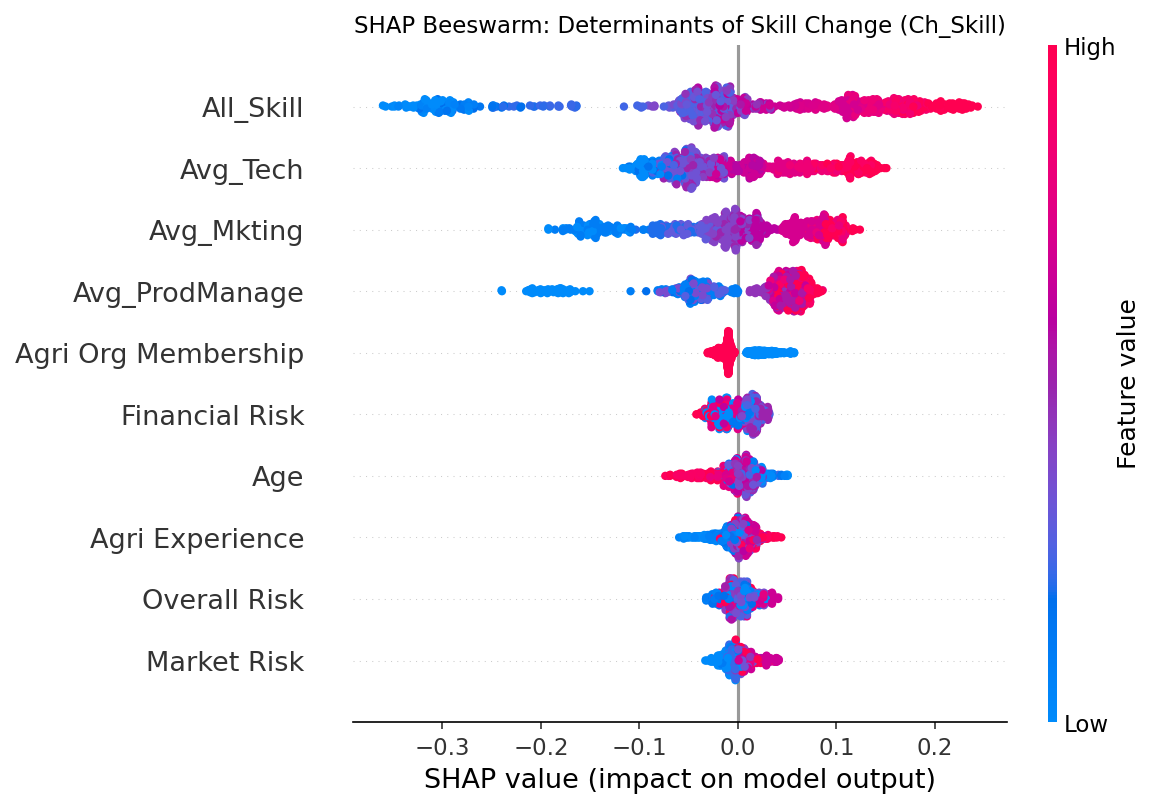
\includegraphics[width=\columnwidth]{figures/fig4_shap_new.png}
\caption{SHAP beeswarm plot showing the distribution and
         direction of feature contributions to individual
         skill improvement predictions.
         Each point represents one observation; colour
         indicates raw feature value (red = high, blue = low).
         Positive SHAP values indicate skill-enhancing
         contributions; negative values indicate
         skill-reducing contributions.}
\label{fig:shap}
\end{figure}

\begin{figure*}[htbp]
\centering
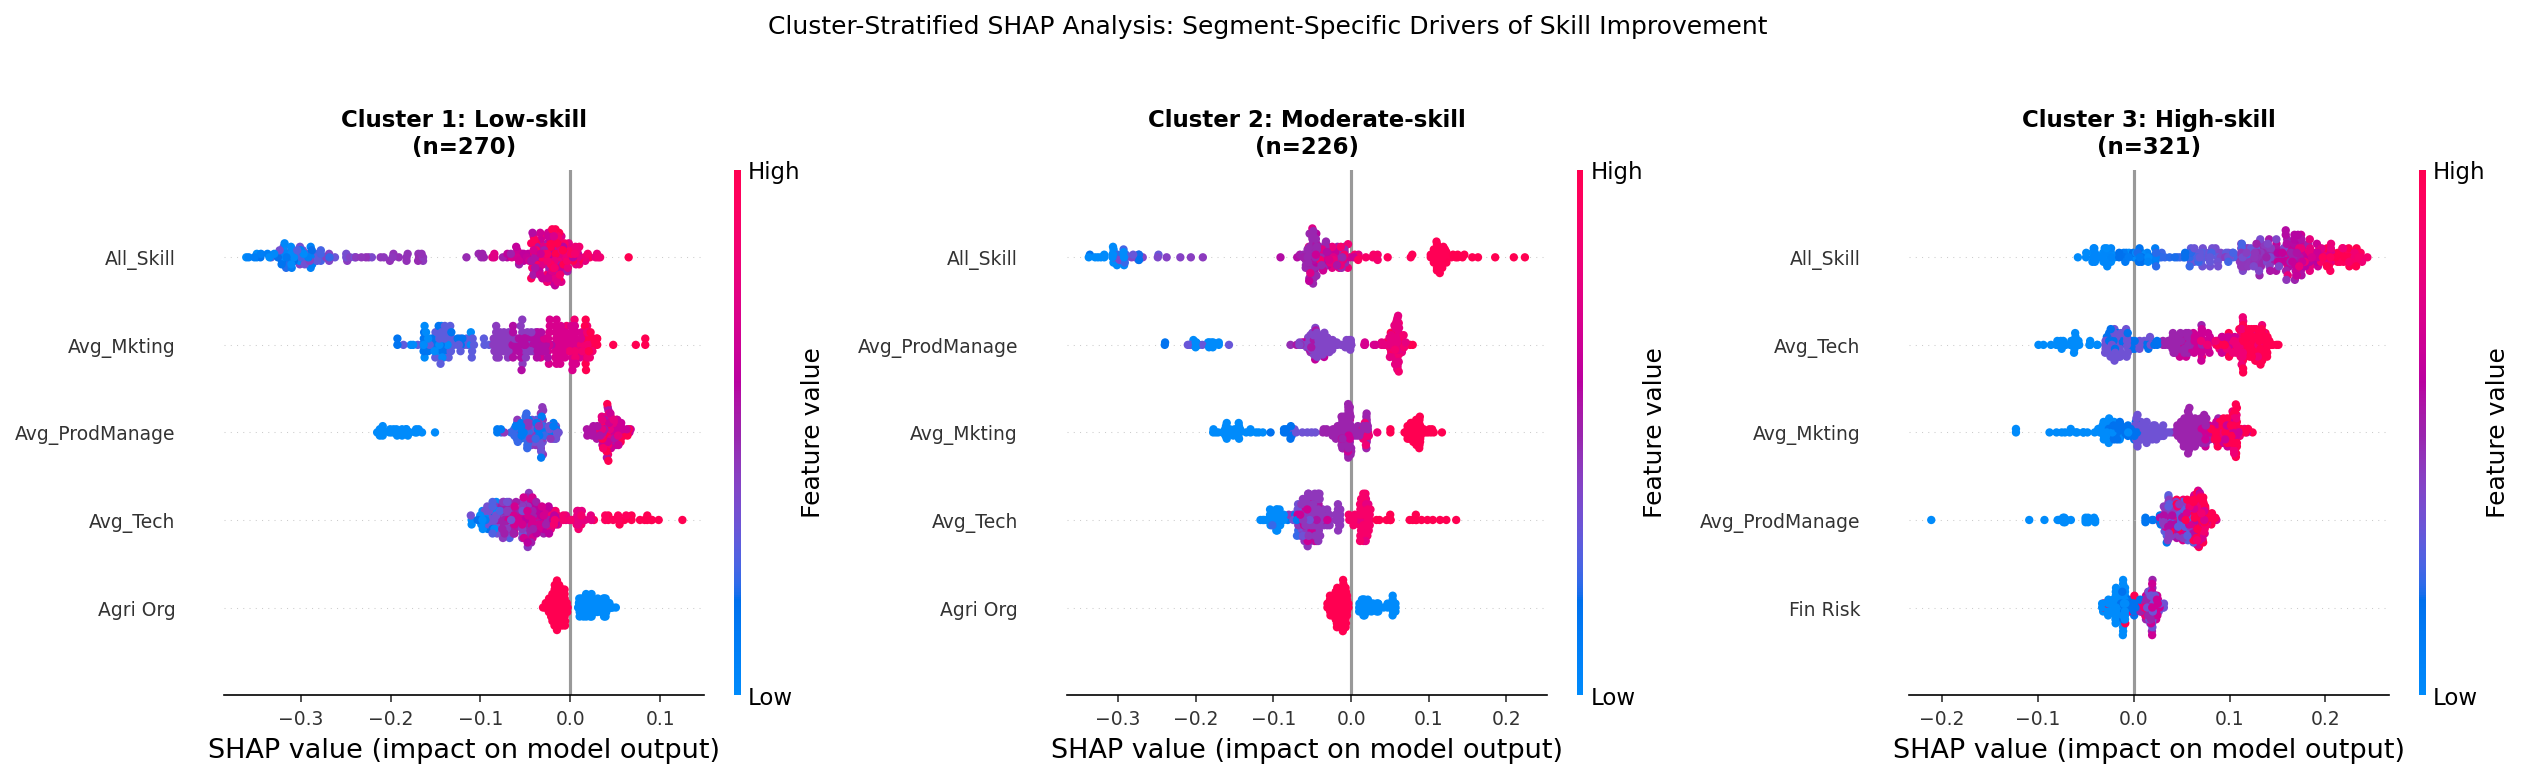
\includegraphics[width=\textwidth]{figures/fig4b_cluster_shap_new.png}
\caption{Cluster-stratified SHAP beeswarm plots for the
         Low-skill (left, $n = 271$),
         Moderate-skill (centre, $n = 228$), and
         High-skill (right, $n = 334$) segments.
         While \texttt{All\_Skill} remains dominant across
         all segments, the relative importance of secondary
         features varies systematically, supporting
         segment-specific training intervention design.}
\label{fig:clusterShap}
\end{figure*}

\begin{figure*}[htbp]
\centering
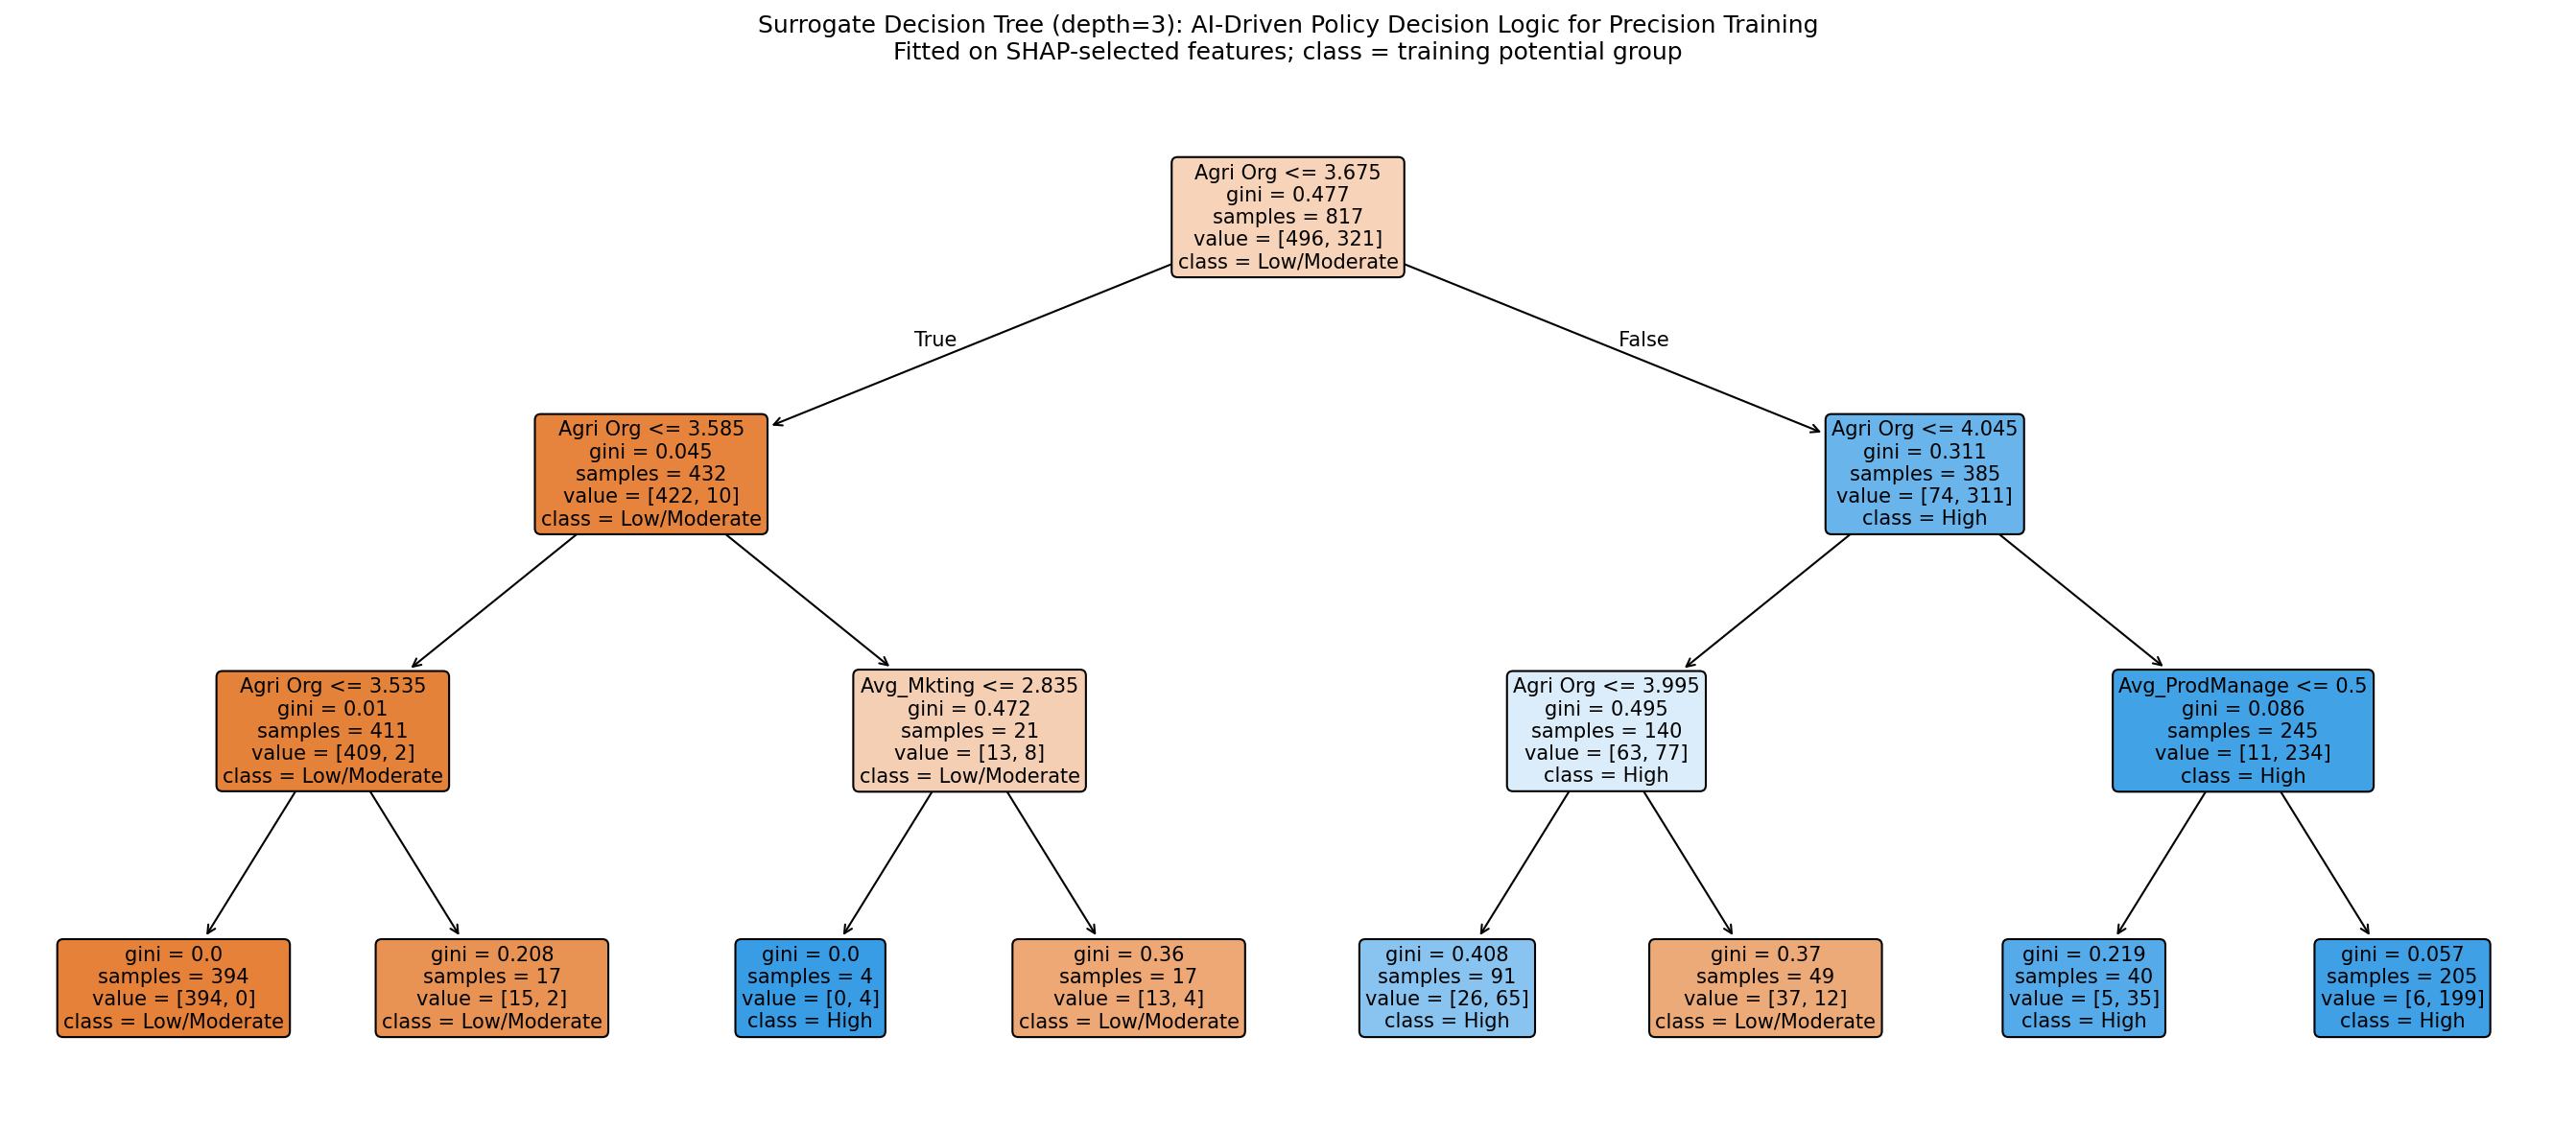
\includegraphics[width=\textwidth]{figures/fig5_rules_new.png}
\caption{Surrogate decision tree (depth = 3, accuracy = 93.3\%,
         $n = 833$) fitted on SHAP-selected features.
         Node labels show the splitting feature and
         data-calibrated threshold, sample count, and class
         distribution (Low/High training potential).
         The tree translates SHAP-derived feature attribution
         into transparent, auditable IF--THEN rules for
         agricultural extension practitioners.}
\label{fig:rules}
\end{figure*}

%%─────────────────────────────────────────────────────────────────────────────
\section{Discussion}
%%─────────────────────────────────────────────────────────────────────────────

\subsection{Predictive Performance in Context}

The optimised Random Forest achieves $R^{2} = 0.213$,
outperforming linear and ridge regression baselines
($R^{2} = 0.185$ and $0.186$, respectively).
This superiority, though modest in absolute terms, is
consistent with the presence of non-linear threshold
effects and feature interactions in the data.
Modest $R^{2}$ values across all models are expected
in observational studies of human behaviour, where skill
change is substantially influenced by unobserved factors
such as motivation, peer effects, and trainer quality
\citep{davis2012}.

Importantly, the framework's value is structural rather than
purely predictive: the Random Forest captures non-linear
patterns that produce meaningful SHAP attributions and
support segment-specific decision rules.
This reinforces the role of explainable machine learning
as a complementary rather than a substitute approach to
linear modelling.

\subsection{Segment-Specific Drivers and the Negative
            Skill Change Finding}

The cluster-level SHAP analysis reveals that the drivers
of skill improvement vary substantively across farmer
segments---a finding that cannot be recovered from global
feature importance alone.
The dominance of \texttt{All\_Skill} across all segments
confirms the central role of pre-training capability as a
moderator of learning outcomes, consistent with human
capital theory \citep{feder1985,davis2012}.

A notable empirical finding is the negative mean skill
change observed in the Low-skill ($Ch\_Skill = -0.233$)
and Moderate-skill ($Ch\_Skill = -0.105$) segments.
Two non-mutually-exclusive mechanisms may explain this pattern.
First, regression-to-the-mean: farmers with the lowest
initial scores are disproportionately likely to score
lower at post-training assessment due to measurement
variance, producing an apparent decline \citep{davis2012}.
Second, selection dynamics: the Smart Farmer program is
voluntary, and Low-skill participants have a
substantially lower participation rate (28.8\%) than
High-skill participants (69.8\%).
The observed skill change in Low-skill farmers therefore
partly reflects the behaviour of non-participants, who
may experience natural skill attrition without structured
training support.
These findings carry direct implications for program
design: they suggest that standard training content alone
is insufficient to produce positive gains in lower-skill
segments, and that foundational scaffolding and targeted
recruitment of low-skill farmers may be prerequisites
for equitable impact.

The rising importance of \texttt{Avg\_Mkting} in the
High-skill segment suggests that market-oriented
competencies become the binding constraint on further
advancement among already high-performing farmers,
pointing toward advanced market-integration training
as the appropriate intervention for this group.

\subsection{Decision Rule Validity and Operationalisability}

The surrogate decision tree provides an interpretable,
data-calibrated representation of the recommendation
logic, achieving 93.3\% classification accuracy.
The primary split at \texttt{All\_Skill} $\leq 3.005$
identifies a threshold below which foundational
training is indicated, covering approximately
26.8\% of the sample.
The two-step extraction process---SHAP for feature
selection, surrogate tree for threshold
calibration---ensures that rules are simultaneously
grounded in attribution theory and optimised for
classification performance.

\subsection{Limitations}

This study is subject to several limitations.
The analysis is based on observational data from a
single national program; all results reflect associative
patterns rather than causal relationships.
The segmentation structure and rule thresholds are
calibrated to this population and may require
recalibration when applied to different agricultural
systems or regions.
The low Silhouette scores reflect overlapping cluster
boundaries that are characteristic of social survey
data; validation with complementary clustering indices
is recommended for future applications.
Future work should pursue prospective validation through
field trials involving extension officers.

%%─────────────────────────────────────────────────────────────────────────────
\section{Conclusion}
%%─────────────────────────────────────────────────────────────────────────────

This study presents an explainable AI-based decision
support system for precision allocation of agricultural
skill development programs, applied to $n = 833$ farmers
in Thailand's Smart Farmer program.
By integrating K-Means segmentation, Random Forest
modelling, and SHAP-based explainability within a unified
SAR pipeline, the framework provides a deployable and
auditable pathway from farmer data to targeted training
recommendations.

The key empirical findings establish that overall skill
level, production management competency, and educational
attainment are the primary determinants of training
effectiveness, with their relative importance varying
systematically across the three farmer segments.
The cluster-level SHAP analysis confirms that global
feature importance is insufficient for precision training
design, and that segment-specific attribution captures
context-dependent learning dynamics that inform practical
and differentiated intervention strategies.

A central methodological contribution is the two-step
rule extraction pipeline: SHAP values identify which
features govern outcomes in each segment, while a
surrogate decision tree (accuracy = 93.3\%) translates
these attributions into optimised, interpretable
classification rules.
This architecture generalises beyond the current
application and can be adapted to any observational
training dataset with pre- and post-assessment measurements.

Future research should explore prospective validation
through quasi-experimental designs, integration with
real-time farmer data streams, and longitudinal tracking
of downstream technology adoption and productivity impacts.
Such developments would strengthen both the causal
foundations and the operational scalability of
AI-driven agricultural extension systems.

%%─────────────────────────────────────────────────────────────────────────────
%% References
%%─────────────────────────────────────────────────────────────────────────────

\begin{thebibliography}{15}
\expandafter\ifx\csname natexlab\endcsname\relax
  \def\natexlab#1{#1}\fi
\providecommand{\url}[1]{\texttt{#1}}
\providecommand{\href}[2]{#2}
\providecommand{\path}[1]{#1}
\providecommand{\doi}[1]{\href{http://dx.doi.org/#1}{\path{#1}}}
\providecommand{\bibinfo}[2]{#2}

\bibitem[{Anderson and Feder(2004)}]{anderson2004}
\bibinfo{author}{Anderson, J.R.}, \bibinfo{author}{Feder, G.},
  \bibinfo{year}{2004}.
\newblock \bibinfo{title}{Agricultural extension: Good intentions and hard
  realities}.
\newblock \bibinfo{journal}{World Bank Research Observer}
  \bibinfo{volume}{19}, \bibinfo{pages}{41--60}.

\bibitem[{Arrieta et~al.(2020)}]{arrieta2020}
\bibinfo{author}{Arrieta, A.B.}, \bibinfo{author}{Diaz-Rodriguez, N.},
  \bibinfo{author}{Del~Ser, J.}, et~al., \bibinfo{year}{2020}.
\newblock \bibinfo{title}{Explainable artificial intelligence (XAI): Concepts,
  taxonomies, opportunities and challenges toward responsible AI}.
\newblock \bibinfo{journal}{Information Fusion} \bibinfo{volume}{58},
  \bibinfo{pages}{82--115}.

\bibitem[{Breiman(2001)}]{breiman2001}
\bibinfo{author}{Breiman, L.}, \bibinfo{year}{2001}.
\newblock \bibinfo{title}{Random forests}.
\newblock \bibinfo{journal}{Machine Learning} \bibinfo{volume}{45},
  \bibinfo{pages}{5--32}.

\bibitem[{Chen and Guestrin(2016)}]{chen2016}
\bibinfo{author}{Chen, T.}, \bibinfo{author}{Guestrin, C.},
  \bibinfo{year}{2016}.
\newblock \bibinfo{title}{XGBoost: A scalable tree boosting system}.
\newblock In: \bibinfo{booktitle}{Proc.\ 22nd ACM SIGKDD},
  pp.\ \bibinfo{pages}{785--794}.

\bibitem[{Davis and Franzel(2012)}]{davis2012}
\bibinfo{author}{Davis, K.}, \bibinfo{author}{Franzel, S.},
  \bibinfo{year}{2012}.
\newblock \bibinfo{title}{Principles for designing and implementing
  agricultural extension programs}.
\newblock \bibinfo{journal}{Journal of Agricultural Education and Extension}
  \bibinfo{volume}{18}, \bibinfo{pages}{249--263}.

\bibitem[{Feder et~al.(1985)}]{feder1985}
\bibinfo{author}{Feder, G.}, \bibinfo{author}{Just, R.E.},
  \bibinfo{author}{Zilberman, D.}, \bibinfo{year}{1985}.
\newblock \bibinfo{title}{Adoption of agricultural innovations in developing
  countries: A survey}.
\newblock \bibinfo{journal}{Economic Development and Cultural Change}
  \bibinfo{volume}{33}, \bibinfo{pages}{255--298}.

\bibitem[{Kamilaris and Prenafeta-Boldu(2018)}]{kamilaris2018}
\bibinfo{author}{Kamilaris, A.}, \bibinfo{author}{Prenafeta-Boldu, F.X.},
  \bibinfo{year}{2018}.
\newblock \bibinfo{title}{Deep learning in agriculture: A survey}.
\newblock \bibinfo{journal}{Computers and Electronics in Agriculture}
  \bibinfo{volume}{147}, \bibinfo{pages}{70--90}.

\bibitem[{Liakos et~al.(2018)}]{liakos2018}
\bibinfo{author}{Liakos, K.G.}, et~al., \bibinfo{year}{2018}.
\newblock \bibinfo{title}{Machine learning in agriculture: A review}.
\newblock \bibinfo{journal}{Sensors} \bibinfo{volume}{18},
  \bibinfo{pages}{2674}.

\bibitem[{Lipton(2018)}]{lipton2018}
\bibinfo{author}{Lipton, Z.C.}, \bibinfo{year}{2018}.
\newblock \bibinfo{title}{The mythos of model interpretability}.
\newblock \bibinfo{journal}{Queue} \bibinfo{volume}{16},
  \bibinfo{pages}{31--57}.

\bibitem[{Lundberg and Lee(2017)}]{lundberg2017}
\bibinfo{author}{Lundberg, S.M.}, \bibinfo{author}{Lee, S.I.},
  \bibinfo{year}{2017}.
\newblock \bibinfo{title}{A unified approach to interpreting model
  predictions}.
\newblock In: \bibinfo{booktitle}{Advances in Neural Information
  Processing Systems (NeurIPS)}.

\bibitem[{Rousseeuw(1987)}]{rouseeuw1987}
\bibinfo{author}{Rousseeuw, P.J.}, \bibinfo{year}{1987}.
\newblock \bibinfo{title}{Silhouettes: A graphical aid to the interpretation
  and validation of cluster analysis}.
\newblock \bibinfo{journal}{Journal of Computational and Applied Mathematics}
  \bibinfo{volume}{20}, \bibinfo{pages}{53--65}.

\bibitem[{Ryo(2022)}]{ryo2022}
\bibinfo{author}{Ryo, M.}, \bibinfo{year}{2022}.
\newblock \bibinfo{title}{Explainable artificial intelligence and interpretable
  machine learning for agricultural data analysis}.
\newblock \bibinfo{journal}{Artificial Intelligence in Agriculture}
  \bibinfo{volume}{6}, \bibinfo{pages}{257--265}.

\bibitem[{Wonggasem et~al.(2024)}]{wonggasem2024}
\bibinfo{author}{Wonggasem, K.}, et~al., \bibinfo{year}{2024}.
\newblock \bibinfo{title}{Automated quality inspection of baby corn using
  image processing and deep learning}.
\newblock \bibinfo{journal}{Artificial Intelligence in Agriculture}
  \bibinfo{volume}{11}, \bibinfo{pages}{61--69}.

\bibitem[{Yang et~al.(2025)}]{yang2025}
\bibinfo{author}{Yang, H.}, et~al., \bibinfo{year}{2025}.
\newblock \bibinfo{title}{AI-driven aquaculture: A review of technological
  innovations and their sustainable impacts}.
\newblock \bibinfo{journal}{Artificial Intelligence in Agriculture}
  \bibinfo{volume}{15}, \bibinfo{pages}{508--525}.

\bibitem[{Zhang et~al.(2026)}]{zhang2026}
\bibinfo{author}{Zhang, T.}, et~al., \bibinfo{year}{2026}.
\newblock \bibinfo{title}{Empowering Chinese medicinal agriculture through
  AI-driven technologies: A comprehensive review}.
\newblock \bibinfo{journal}{Artificial Intelligence in Agriculture}.

\end{thebibliography}

\end{document}
